\documentclass[a4paper, 10pt]{article}

\usepackage[utf8]{inputenc}
\usepackage[italian]{babel}
\usepackage[T1]{fontenc}
\usepackage{csquotes}

\usepackage[colorlinks=true]{hyperref}

\usepackage{datetime2}
\usepackage{enumitem}

\usepackage{graphicx}
\usepackage{subcaption}


% change datetime2 settings
\DTMsetdatestyle{ddmmyyyy}
\DTMsetup{datesep=/}

\usepackage{minted}
\usemintedstyle{one-dark}

\usepackage{biblatex}
\addbibresource{citations.bib}



% count within section
\counterwithin{figure}{section}
\counterwithin{listing}{section}

\newcommand{\lenet}{LeNet\(5\)+}


\begin{document}

\title{\textsc{Risolutore di sudoku in Python con OpenCV e Keras}}
\author{Simone Fidanza}
\date{\today}


\maketitle

\begin{abstract}
    Per estrarre la griglia di un sudoku da un'immagine dello stesso è stata
    utilizzata la libreria OpenCV, in seguito le singole cifre sono state
    analizzate dalla Convolutional Neural Network ispirata al modello LeNet5.
    Dopo aver predetto le cifre e aver costruito una griglia artificiale di
    numeri, il sudoku viene risolto da un'algoritmo.
\end{abstract}


\section{Introduzione}\label{sec:introduzione}

L'obiettivo ultimo dell'applicazione è quello di risolvere un sudoku da
un'immagine. Per poter fare ciò sono necessari diversi passaggi:

\begin{enumerate}
    \item Fornire un'immagine in input contenente un sudoku;
    \item Localizzare la griglia del sudoku e estrarla;
    \item Data la griglia, individuare ogni singola cella della stessa;
    \item Determinare se la cella contiene una cifra e se sì effettuare il
        riconoscimento ottico dei caratteri (per brevità OCR);
    \item Risolvere il sudoku mediante un algoritmo;
    \item Mostrare il sudoku risolto all'utente.
\end{enumerate}

L'applicazione fa ampio utilizzo delle librerie OpenCV\footnote{acronimo in
lingua inglese di \emph{Open Source Computer Vision Library}
}~\cite{opencv_library}, TensorFlow~\cite{tensorflow2015-whitepaper},
Keras~\cite{chollet2015keras} e NumPy~\cite{harris2020array}.


\section{Localizzazione della griglia}

Come prima cosa, dopo aver ricevuto l'immagine di un sudoku in input, è
necessario individuare la griglia del sudoku e per farlo è stata utilizzata la
libreria OpenCV. L'immagine iniziale subisce una serie di passaggi, ovvero:

\begin{itemize}
    \item viene convertita in scala di grigi con
        \mintinline{py3}{cv2.cvtColor()};
    \item viene applicata una sfocatura Gaussiana con
        \mintinline{py3}{cv2.GaussianBlur()} per renderla più uniforme;
    \item viene segmentata con
        \mintinline{py3}{cv2.adaptiveThreshold()}\footnote{è stata preferita
        una soglia adattiva per conservare quanti dettagli possibile
        dell'immagine} per trasformarla in un'immagine binaria;
    \item viene invertita con \mintinline{py3}{cv2.bitwise_not()};
    \item viene infine erosa con \mintinline{py3}{cv2.erode()} e
        successivamente dilatata con \\ \mintinline{py3}{cv2.dilate()} per
        rimuovere il rumore presente nell'immagine.
\end{itemize}

\begin{figure}[ht]
    \def\subwidth{0.40}
    \def\imgwidth{0.70}
    \centering
    \begin{subfigure}[b]{\subwidth\linewidth}
        \centering
        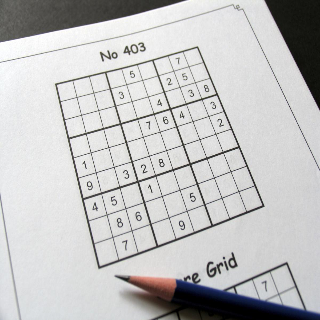
\includegraphics[width=\imgwidth\linewidth]{imgs/input.png}
        \caption{Originale}\label{subfig:input}
        \vspace{4ex}
    \end{subfigure}%%
    \begin{subfigure}[b]{\subwidth\linewidth}
        \centering
        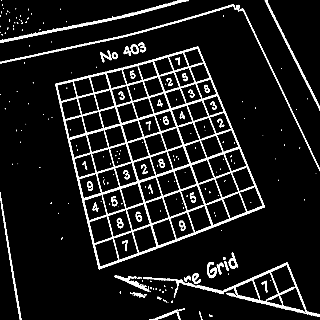
\includegraphics[width=\imgwidth\linewidth]{imgs/process_out.png}
        \caption{Pre-elaborazione}\label{subfig:preprocess}
        \vspace{4ex}
    \end{subfigure}
    \begin{subfigure}[b]{\subwidth\linewidth}
        \centering
        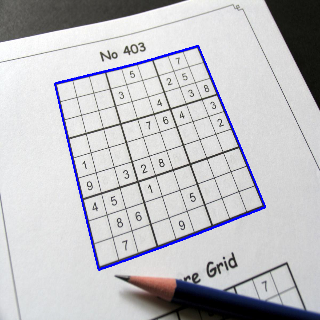
\includegraphics[width=\imgwidth\linewidth]{imgs/grid.png}
        \caption{Griglia}\label{subfig:grid}
    \end{subfigure}%%
    \begin{subfigure}[b]{\subwidth\linewidth}
        \centering
        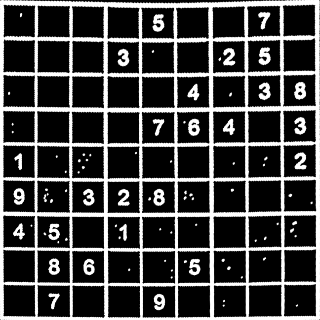
\includegraphics[width=\imgwidth\linewidth]{imgs/warp.png}
        \caption{Deformazione}\label{subfig:warp}
    \end{subfigure}
    \caption{Processo di estrazione della griglia di un sudoku}\label{fig:extraction}
\end{figure}

Il risultato di questi passaggi è illustrato in figura~\ref{subfig:preprocess}.
Dopo che l'immagine è stata pre-elaborata, si può procedere all'estrazione
della griglia.

Innanzitutto è necessario individuare il bordo della griglia. È stato supposto
che questo sia il più grande tra i bordi che la funzione
\mintinline{py3}{cv2.findContours()} restituirà, come illustrato in
figura~\ref{subfig:grid}.
Approssimando il bordo con \\ \mintinline{py3}{cv2.approxPolyDP()} è possibile
ottenere gli angoli della griglia.
Usando sia quest'ultimi che \mintinline{py3}{cv2.getPerspectiveTransform()} che \mintinline{py3}{cv2.WarpPerspective()} l'immagine viene deformata e resa piana,
come illustrato in figura~\ref{subfig:warp}.


\section{Analisi delle celle}

Per determinare se una cella contiene un numero o meno è necessario innanzitutto
estrarre le singole celle dalla griglia piana. Per fare ciò, sono state divise
per \(9\) le dimensioni della griglia e sono state estratte \(81\) celle di tali
dimensioni. Attraverso un semplice algoritmo viene verificato se la cella
contiene un numero o meno. Se la cella contiene un numero, questo viene
estratto e analizzato dalla rete neurale, la predizione viene inserita nella
lista rappresentante la griglia del sudoku. Se la cella non contiene un numero,
nella lista viene inserito il numero \(0\).


\section{Modello}

Per poter effettuare l'OCR è necessario un modello di Machine Learning. Il
modello proposto è un miglioramento della rete neurale
LeNet5~\cite{lecun1998gradient}. Il modello non è altro che una semplice
Convolutional Neural Network (CNN per brevità) che è stata allenata sul dataset
MNIST~\cite{deng2012mnist} che contiene \(60,000\) immagini per l'allenamento e
\(10,000\) per l'analisi. Il modello è illustrato in
figura~\ref{fig:architecture}. \\

\begin{figure}[h]
    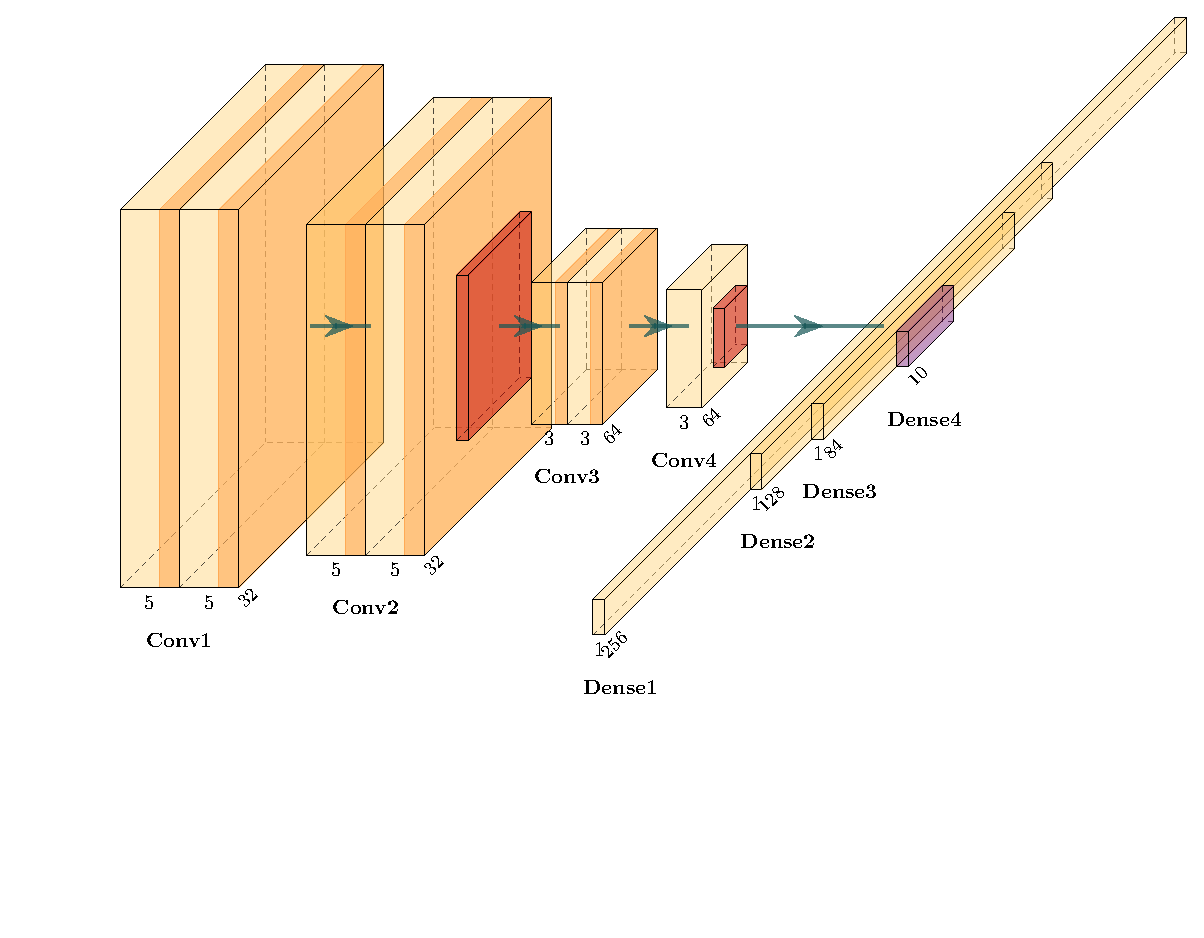
\includegraphics[width=0.9\textwidth, trim = 1cm 4.5cm 0cm 1cm]{architecture.pdf}
    \caption{Architettura della rete neurale \lenet. Ogni piano rappresenta un
    layer della Rete Neurale.}\label{fig:architecture}
\end{figure}

Per allenare \lenet{} è stato utilizzato un tasso di apprendimento variabile.
Nel momento in cui il modello registra che l'apprendimento è ``stagnante'', il
tasso dello stesso viene ridotto di \(0.2\) attraverso la classe
\mintinline{py3}{ReduceLROnPlateau()} del modulo \mintinline{py3}{callbacks}
di \mintinline{py3}{keras}.
Utilizzando l'accorgimento precedente e allenando il modello per \(30\) epoche,
con una dimensione del lotto di \(86\), esso ha raggiunto un'accuratezza del
\(\approx 99.67\%\).

\section{Risoluzione del sudoku}

Dopo aver estratto le cifre dalla griglia e aver formato una griglia
``digitale'' del sudoku, quest'ultima viene passata alla funzione
\mintinline{py3}{SudokuSolver.solve()} che risolve il sudoku. Infine viene
stampata schermo la soluzione.

\section{Limitazioni conosciute}

Poiché l'algoritmo di estrazione della griglia non è perfetto, seguono le
limitazioni conosciute:

\begin{itemize}
    \item nel deformare e appiattire un'immagine già piana, questa viene ruotata di \(90^\circ\) in senso orario. Per ovviare a questo inconveniente, è stata aggiunta una rotazione in senso antiorario;
    \item nel determinare se una cella è priva o meno di numero, poiché l'algoritmo si basa sul numero di pixel bianchi, a volte l'algoritmo può ignorare celle che contengono dei numeri. Per questo motivo la funzione \mintinline{py3}{SudokuExtractor.construct_board()} accetta un parametro opzionale che è proprio il valore minimo di pixel bianchi;
    \item nel predirre le cifre, la rete neurale confonde il numero \(1\) col numero \(7\) e raramente il numero \(6\) col numero \(5\) o \(8\)\footnote{questo accade quando la parte superiore del numero \(6\) è troppo incurvata verso il basso}
\end{itemize}


\bigskip
\printbibliography

\end{document}
